% !TEX root =  paper.tex

\section{Related Work}
% \begin{figure}[t]
%  	\subfloat[]{
%  		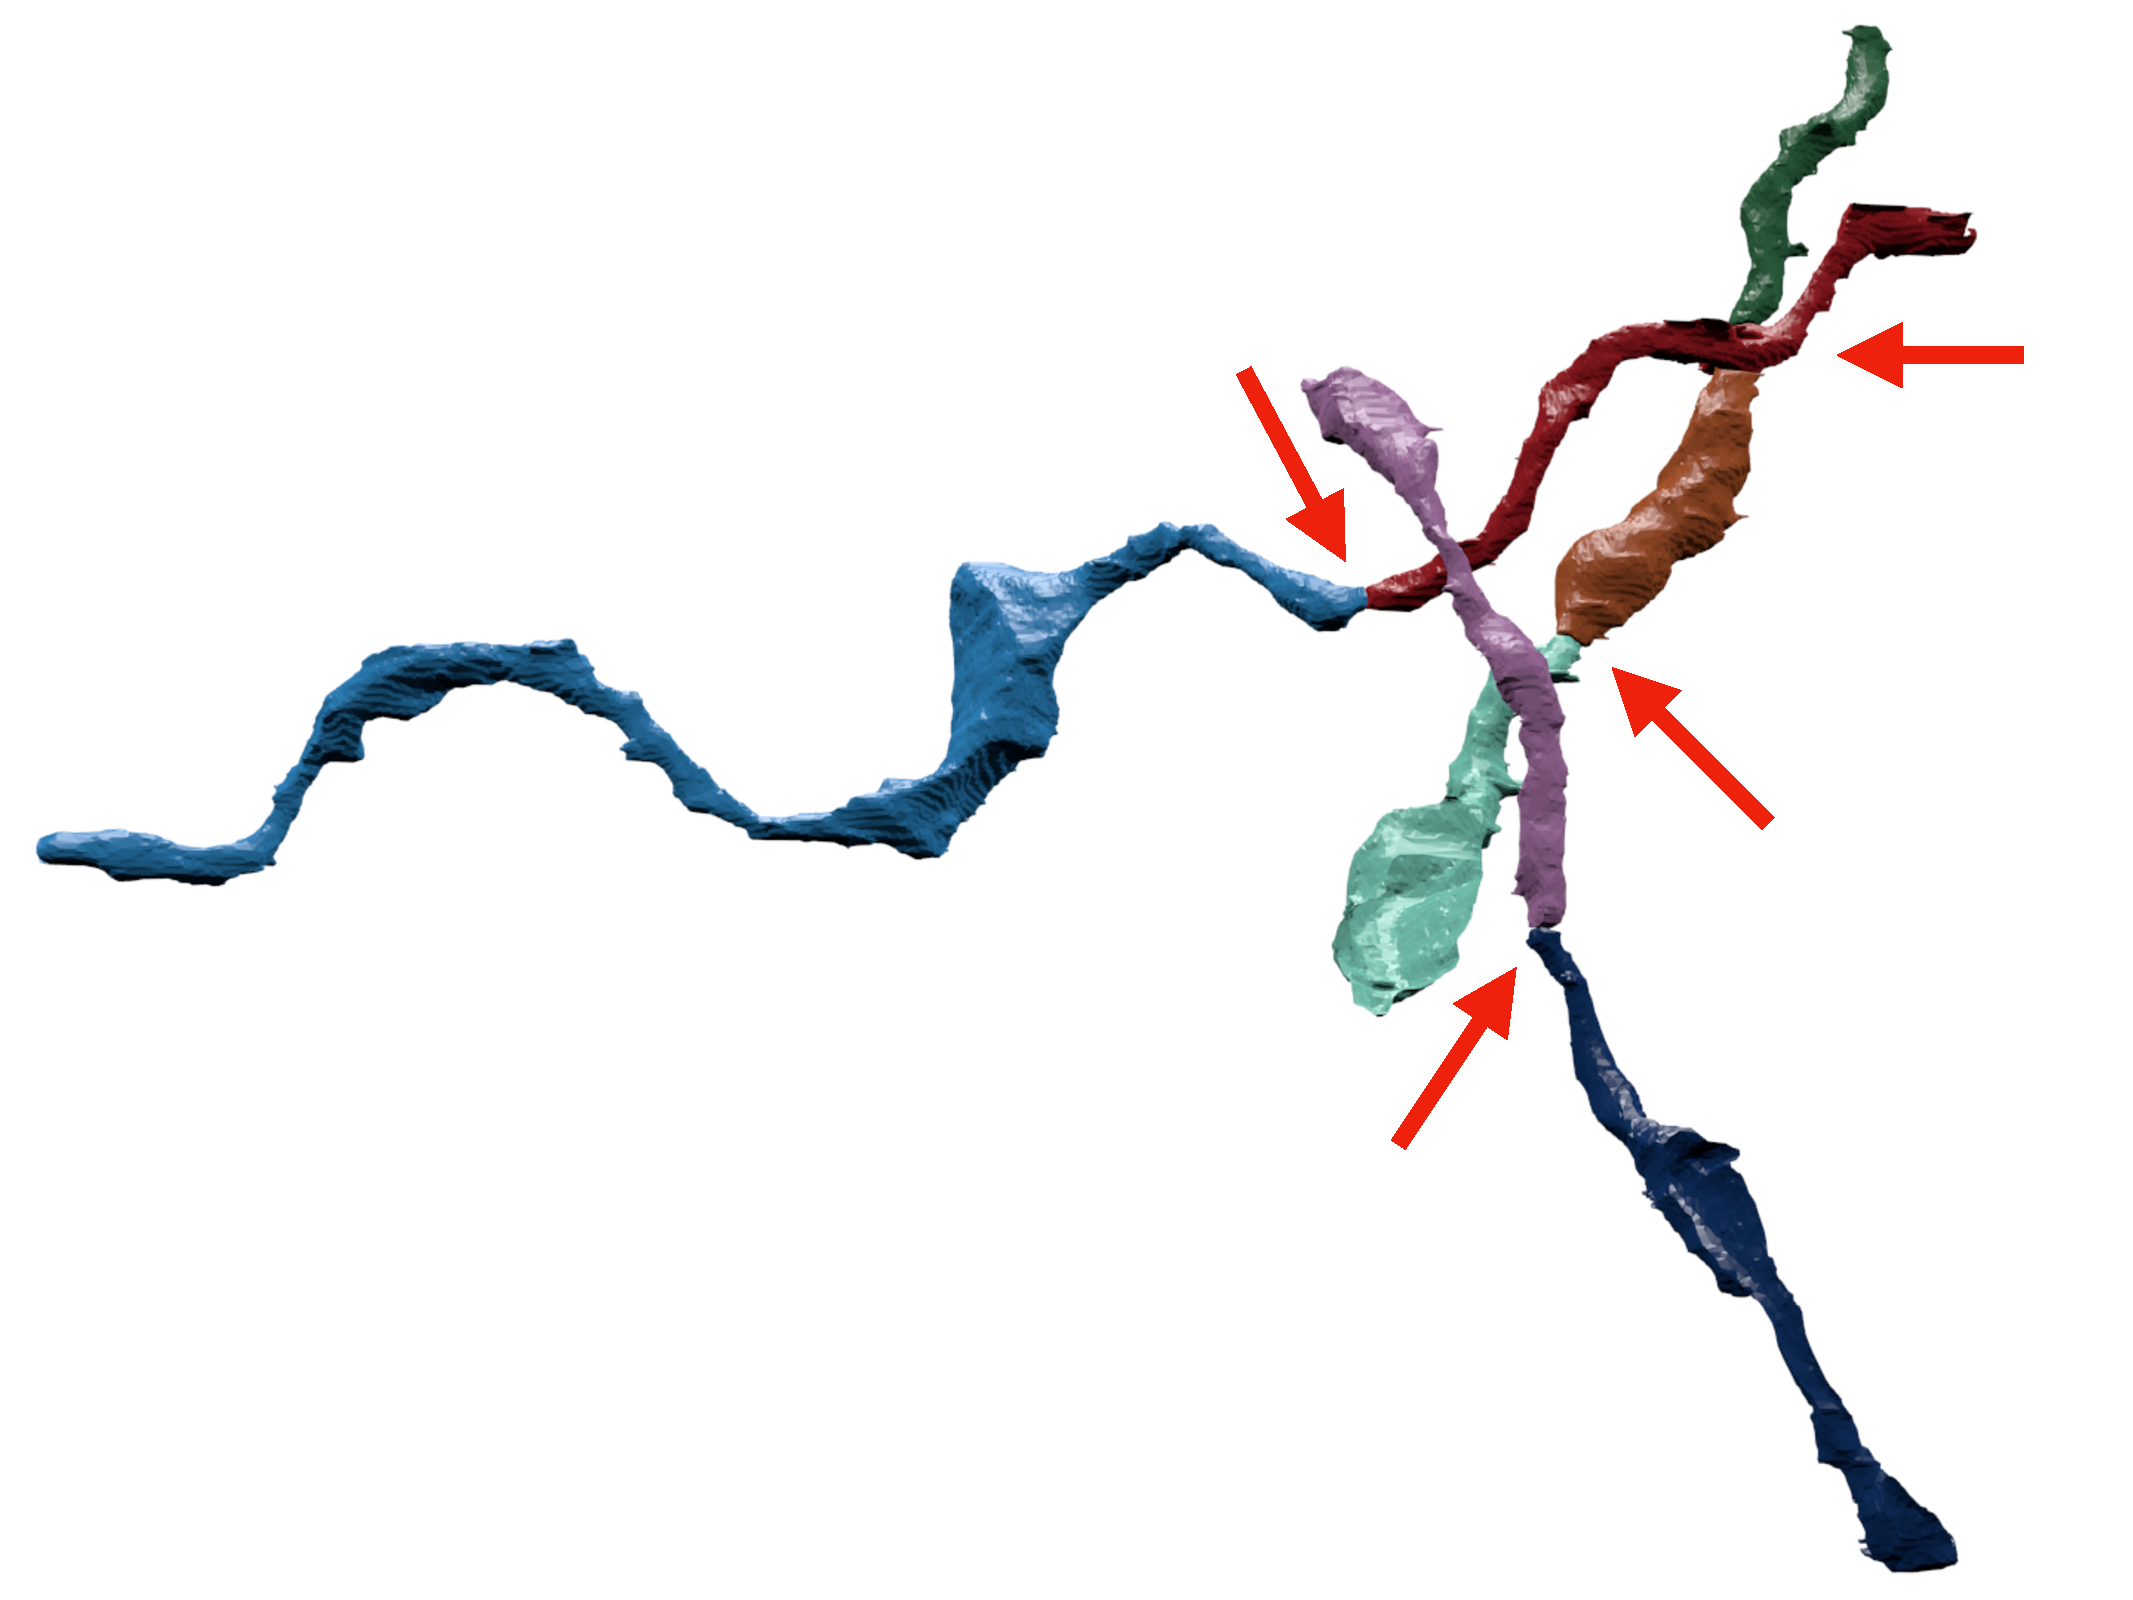
\includegraphics[width=.47\linewidth]{figures/schema/pre-multicut-with-arrows.pdf}
%  	}
%  	\subfloat[]{
%  		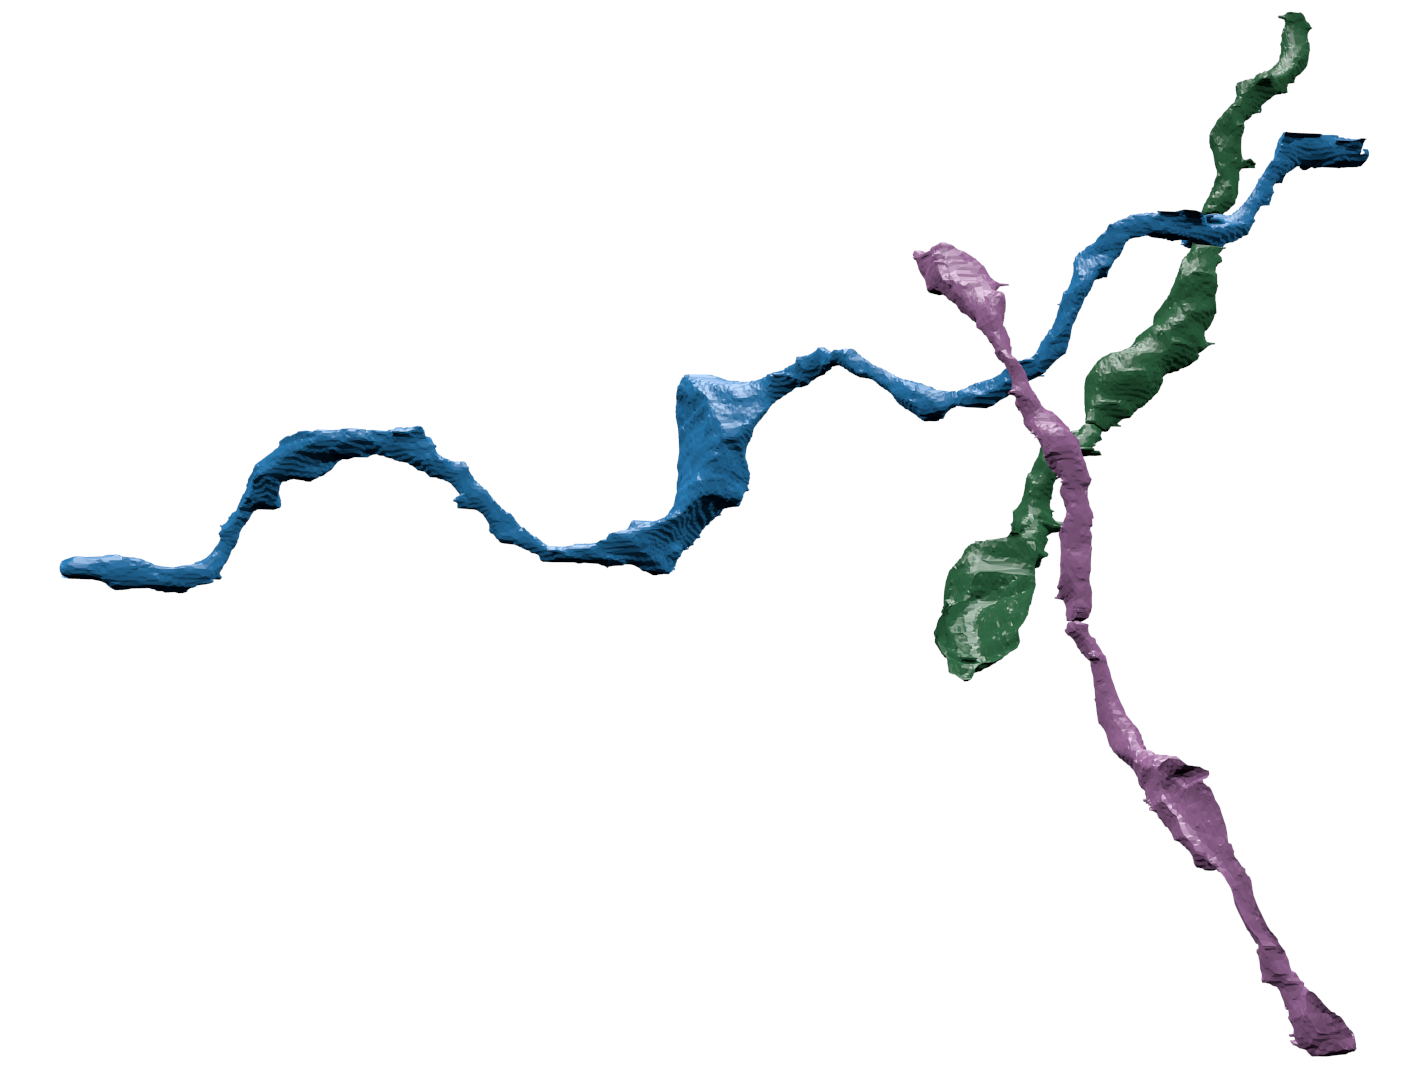
\includegraphics[width=.47\linewidth]{figures/schema/post-multicut.png}
%  	}
%  	\caption{Example improvement of neural reconstruction. (a) We extract 3D skeletons from pixel-based segmentation algorithms to create a graph representation. Red arrows highlight errors in the input segmentation. (b) We improve the segmentation accuracy using a graph partitioning algorithm, leveraging both local and global information.}
%  	\label{fig:improved-reconstruction}
% \end{figure}
%\\~\\
\noindent\textbf{Pixel-Based Segmentation}
%\subsubsection{Pixel-Based Segmentation}
A significant amount of connectomics research considers the problem of extracting segmentation information at the voxel level of EM images.
First, intermediate representations like boundary, affinity or binary segmentation maps are generated from the voxels.
Random forests with hand-designed features~\cite{kaynig2015large}, or 2D and 3D convolutional networks produce boundary probabilities. ~\cite{seymour2016rhoananet,ronneberger2015u,bogovic2013learned,ciresan2012deep,jain2010boundary,amelio_segmentation}.
Often, the affinity between each voxel and its six neighbors are used~\cite{lee2015recursive,parag2017anisotropic,lee2017superhuman,cciccek20163d,turaga2010convolutional}. 
The 3D U-Net architecture has become popular~\cite{cciccek20163d} and the MALIS cost function is specifically designed to re-weight affinity predictions by their contribution to the segmentation error~\cite{briggman2009maximin}.
More recently, flood-filling networks~\cite{januszewski2016flood} produce binary segmentations from raw pixels with a recurrent convolutional network at a high computational cost.
Orthogonal to the representation, model averaging~\cite{zeng2017deepem3d} and data augmentation~\cite{lee2017superhuman} methods can further improve the performance, where Lee et al.~\cite{lee2017superhuman} surpass the estimated human accuracy on the SNEMI3D dataset.

Clustering techniques transform these intermediate representations into segmentations.
Some early methods apply computationally expensive graph partitioning algorithms with a single node per superpixel~\cite{andres2012globally}.
Several pixel-based approaches generate probabilities that neighboring pixels belong to the same neuron.
Often a watershed algorithm will then cluster these pixels into super-pixels~\cite{zlateski2015image}.
\\~\\
\noindent\textbf{Region Merging}
%\subsubsection{Region Merging}
Region merging methods can be categorized by the similarity metric between adjacent segments and the merging strategy.
For the similarity metric, Lee et al. and Funke et al. rely solely on the accuracy of the predicted affinities and define the metric as the mean affinity between segments~\cite{lee2017superhuman,funke2017deep}.
Classification-based methods generate the probability to merge two segments from handcrafted~\cite{seymour2016rhoananet,nunez2014graph,parag2017anisotropic,zlateski2015image,10.1371/journal.pone.0125825,jain2011learning} and learned features~\cite{bogovic2013learned}. 
For the merging strategy, most methods use variants of hierarchical agglomeration ~\cite{seymour2016rhoananet,nunez2014graph,parag2017anisotropic,zlateski2015image,10.1371/journal.pone.0125825} to greedily merge a pair of regions at a time.
Jain et al. formulates the agglomeration problem as a reinforcement learning problem ~\cite{jain2011learning} and Pape et al. present a scalable multicut algorithm to partition superpixels with global optimization~\cite{beier2017multicut}.
\\~\\
\noindent\textbf{Error-correction Methods}
 Additional research builds on top of these region-based methods to correct errors in the segmentation. This can be done either using human proofreading~\cite{haehn2014design,haehn2017guided,mojo2} or automatically~\cite{rolnick2017morphological,error_correction_using_CNN}. In both cases, available methods are pixel-based and do not include global biological constraints into the decision making process.  
% Many segmentation and clustering algorithms use graph partitioning techniques~\cite{andres2012globally} or normalized cuts for traditional image segmentation~\cite{kappes2016higher,shi2000normalized,tatiraju2008image}.




% Even though graph partitioning is an NP-Hard problem~\cite{demaine2006correlation} there are several useful multicut heuristics that provide good approximations with reasonable computational costs~\cite{horvnakova2017analysis}. 
%We extract a 3D graph from an input segmentation for a true top-down error correction approach. 
%This allows us to enforce domain-specific biological constraints while using graph partitioning algorithms. 
%We use the method of Keuper et al.~\cite{keuper2015efficient} to partition the extracted graph into the final neural reconstruction.

%\subsubsection{Error-correction methods}
%Additional research builds on top of these region-based methods to correct errors in the segmentation either using human proofreading~\cite{haehn2014design,haehn2017guided,mojo2} or automatic methods~\cite{rolnick2017morphological,error_correction_using_CNN}.
%However, to our knowledge, our method is the first to extract a 3D graph from an input segmentation for a true top-down\TODO{?} error correction approach. 
%This allows us to enforce domain-specific biology constraints and use efficient graph partitioning algorithms. 
% Many segmentation and clustering algorithms use graph partitioning techniques~\cite{andres2012globally} or normalized cuts for traditional image segmentation~\cite{kappes2016higher,shi2000normalized,tatiraju2008image}.
% Even though graph partitioning is an NP-Hard problem~\cite{demaine2006correlation} there are several useful multicut heuristics that provide good approximations with reasonable computational costs~\cite{horvnakova2017analysis}. 
%We use the method of Keuper et al.~\cite{keuper2015efficient} to partition the extracted graph into the final neural reconstruction.

